\documentclass{standalone}
\usepackage{tikz}
\makeatletter\AtBeginDocument{\@buildstepset{1,2,3,4,5,6}}\makeatother
\usetikzlibrary{intersections, calc}
\usepackage{hsbcommon}
    \begin{document}
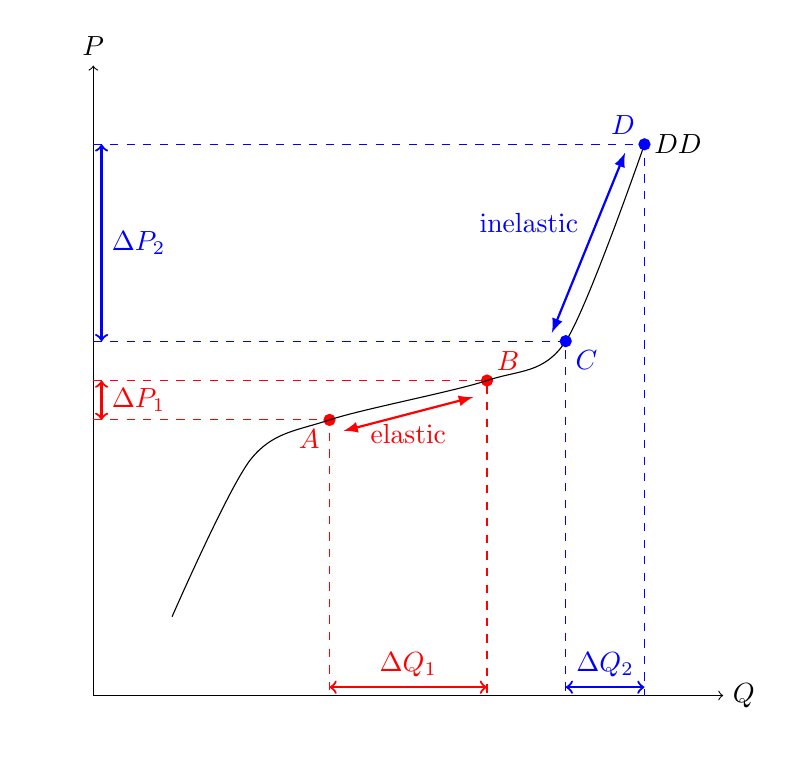
\begin{tikzpicture}
        \draw[->] (0,0) node[below] {\phantom{$X_i$}} -- (8,0) node[right] (Q) {$Q$};
        \draw[->] (0,0) node[left] {\phantom{$Y_mi$}} -- (0,8) node[above] (P) {$P$};

        % \coordinate (A) at (1,7);
        % \coordinate (B) at (2,6.7);
        % \coordinate (C) at (3,6);
        % \coordinate (D) at (4,3);
        % \coordinate (E) at (6,2.2);
        % \coordinate (F) at (7,1.7);

              \coordinate (A) at (1,1);
            \coordinate (B) at (2,3);
            \coordinate (C) at (3,3.5);
            \coordinate (D) at (5,4);
            \coordinate (E) at (6,4.5);
            \coordinate (F) at (7,7);

        \ifstep{1}{
\begin{scope}[color=red]

            \filldraw (C) circle (2pt) node[below left] {$A$};
            \filldraw (D) circle (2pt) node[above right] {$B$};

            \draw[dashed]  (0, |- C) -- (C) -- (C |-,0);
            \draw[dashed]  (0, |- D) -- (D) -- (D |-,0);

            \draw[thick, <->,xshift=3pt] (0, |- C) -- node [right] {$\Delta P_1$} (0, |- D);
            \draw[thick, <->,yshift=3pt] (C |-,0) -- node [above] {$\Delta Q_1$} (D |-,0);

            \draw[thick, <->, >=latex] ([xshift=5pt,yshift=-4pt] C) -- node [below] {elastic} ([xshift=-5pt,yshift=-6pt] D);
            
        \end{scope}
}

        
        \draw [name path=demand] plot [smooth] coordinates {(A) (B) (C) (D) (E) (F)};
        \node[right] at (F) {$DD$};

        % \node at (5,8) {\parbox{20ex}{between $A$ and $B$: inelastic demand}};
        
        \ifstep{2}{
\begin{scope}[color=blue]

            \filldraw (E) circle (2pt) node[below right] {$C$};
            \filldraw (F) circle (2pt) node[above left] {$D$};

            \draw[dashed]  (0, |- F) -- (F) -- (F |-,0);
            \draw[dashed]  (0, |- E) -- (E) -- (E |-,0);
            
            \draw[thick, <->,xshift=3pt] (0, |- F) -- node [right] {$\Delta P_2$} (0, |- E);
            \draw[thick, <->,yshift=3pt] (F |-,0) -- node [above] {$\Delta Q_2$} (E |-,0);
            
            \draw[thick, <->, >=latex] ([xshift=-7pt,yshift=-3pt] F) -- node [above left] {inelastic} ([xshift=-5pt,yshift=3pt] E);

            % \coordinate (G) at (1,1);
            % \coordinate (H) at (2,3);
            % \coordinate (I) at (3,3.5);
            % \coordinate (J) at (5,4);
            % \coordinate (K) at (6,4.5);
            % \coordinate (L) at (7,7);
            
            % \draw [name path=supply] plot [smooth] coordinates {(G) (H) (I) (J) (K) (L)};
            % \node[right] at (L) {$SS$};
    
                
            % \path [name intersections={of=demand and supply,by=X}];
    
            % \filldraw (X) circle (2pt);
    
            % \draw[dashed]  (0, |- X) -- (X) -- (X |-,0);
            
        \end{scope}
}

 
        
    \end{tikzpicture}
\end{document}
